\tikzset{
  estilo nodos/.style={
      node distance=2.5cm,
      estado/.style={circle, draw, minimum size=1cm, inner sep=0pt},
      proba/.style={-latex, thin, bend left=20pt},
      every node/.style={font={\tiny}},
    },
  add flechas/.code={
      \draw[proba] (0) to node[above] {rec.} (1);
      \draw[proba] (1) to node[above] {rec.} (2);
      \draw[proba] (2) to node[above] {$\dots$} (dots.north west);
      \draw[proba] (dots.north east) to node[above] {$\dots$} (n-2);
      \draw[proba] (n-2) to node[above] {rec.} (n-1);
      \draw[proba] (n-1) to node[above] {rec.} (n);
    },
}

\begin{enunciado}{\ejercicio[PotenciaSum]}
  \textit{PotenciaSum}

  Suponga que se tiene un método \textit{potencia} que, dada una matriz cuadrada $A$ de orden $4 \times 4$ y un número $n$,
  computa la matriz $A^n$. Dada una matriz cuadrada $A$ de orden $4 \times 4$ y un número natural $n$ que es potencia de 2
  (i.e, $n = 2^k$ para algún $k \geq 1$), desarrollar, utilizando la técnica de dividir y conquistar y el método \textit{potencia},
  un algoritmo que permita calcular
  $$
    A^1 + A^2 + A^3 + \cdots + A^n.
  $$
  Procure que el algoritmo propuesto aplique el método $potencia$, sume y haga productos de matrices una cantidad estrictamente menor que
  $O(n)$ veces.
\end{enunciado}

\textit{¿Qué ondis?}
Para tener en mente: Si tengo que implementar \textit{divide \& conquer} y además tener un \textit{running time} menor a $O(n)$,
seguramente me están pidiendo que la complejidad sea $O(\log(n))$, lo cual implicaría un árbol de una rama $\log_2(n)$ niveles, dividiendo
al input a la mitad en cada iteración.

Intento ver si puedo factorizar para calcular esto en forma recursiva:

Dado que $n \en \set{2, 4, 8, \ldots, 2^k}$, el caso base sería con $n = 2$:
{\small
$$
  \begin{array}{rcl}
    n = 2 & \entonces & A + A^2 = \ob{A \cdot (I + A)}{\text{caso base}} \\
    n = 4 & \entonces &
    A + A^2 + A^3 + A^4 =
    A \cdot (I + A + A^2 + A^3) =
    A \cdot (I + A \cdot (I + A + A^2)) =
    A \cdot (I + A \cdot (I + \ub{A \cdot (I + A)}{\text{caso base}}))
  \end{array}
$$
}
Ahí hay un patrón recursivo de esta pinta:
$$
  \textit{\green{potSum}}(A, n) =
  \llave{ccl}{
    A \cdot (I + A) & \text{si} & n = 2\\
    A \cdot (I + \textit{\green{potSum}}(A, \frac{n}{2})) & \text{si} & n > 2
  }
$$

$$
  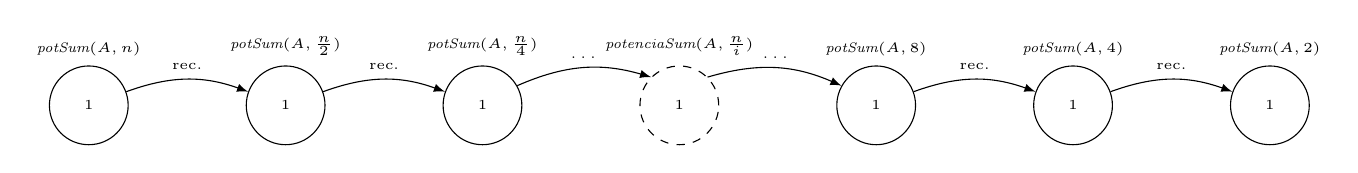
\begin{tikzpicture}[estilo nodos]
    \node[estado, label=above:{$\textit{\green{potSum}}(A,n)$}] (0) {$1$};
    \node[estado, right of=0, label=above:{$\textit{\green{potSum}}(A,\frac{n}{2})$}] (1) {$1$};
    \node[estado, right of=1, label=above:{$\textit{\green{potSum}}(A,\frac{n}{4})$}] (2) {$1$};
    \node[estado, right of=2, label={$\textit{\green{potenciaSum}}(A,\frac{n}{i})$}, dashed] (dots) {$1$};
    \node[estado, right of=dots, label=above:{$\textit{\green{potSum}}(A,8)$}] (n-2) {$1$};
    \node[estado, right of=n-2, label=above:{$\textit{\green{potSum}}(A,4)$}] (n-1) {$1$};
    \node[estado, right of=n-1, label=above:{$\textit{\green{potSum}}(A,2)$}] (n) {$1$};

    \draw[proba] (0) to node[above] {rec.} (1);
    \draw[proba] (1) to node[above] {rec.} (2);
    \draw[proba] (2) to node[above] {$\dots$} (dots.north west);
    \draw[proba] (dots.north east) to node[above] {$\dots$} (n-2);
    \draw[proba] (n-2) to node[above] {rec.} (n-1);
    \draw[proba] (n-1) to node[above] {rec.} (n);
  \end{tikzpicture}
$$

Árbol de una sola rama, dado que la función tiene una sola llamada recursiva en cada llamada ¿Cuántos niveles tiene el árbol?
¡Busco la cantidad de iteraciones $k$ hasta llegar al caso base $n=2$!:
$$
  \textstyle
  T(A, \frac{n}{2^k}) \igual{\red{!}} T(A, 2)
  \sii
  \frac{n}{2^k} = 2
  \sii
  n = 2^{k+1}
  \sii
  \log_2(n) = k + 1
  \sii
  k = \log_2(n) - 1
$$
Los subproblemas tienen un costo constante porque las matrices tienen un tamaño constante de $4 \times 4$, por eso le puse un $1$ a los nodos
del árbol. Por lo tanto estoy sumando 2 matrices y multiplicando 2 matrices por cada subproblema, lo cual es algo constante así que \sout{me chupa
  un huevo} no aporta nada. La complejidad o \textit{running time} de este algoritmo \textit{\green{potSum}}:
$$
  \cajaResultado{
    T(n) \en \Theta(\log(n))
  }
$$

Un pseudocódigo para pasar a la compu:
\begin{tcolorbox}
  \begin{lstlisting}[
      mathescape=true,
      emph={[1]funcion, return, ret, retorno},
      emph={[2]si, sino, if, else},
      emph={[3]potencia, potSum},
      emphstyle={[1]\color{violet}\it},
      emphstyle={[2]\color{red}\it},
      emphstyle={[3]\color{OliveGreen}\it},
      morecomment={[l]{//}},
      commentstyle={\color{gray}\it\footnotesize}
  ]
 funcion potSum(A, n)
     si n = 2
         ret A$\cdot$(I+A)  // O(1)
     m <- n/2
     B <- potSum(A,m)
     ret A$\cdot$(I+B)      //O(1)\end{lstlisting}
\end{tcolorbox}

{\tiny
Todo parece fácil ahora, pero antes de darme cuenta que la cosa iba por el lado de la recursión y no por el lado de resolver el problema
encontrando un súper hack,  estuve un día entero falopeando esto:

Haciendo muchas factorizaciones en grupos llegué a esto:
$$
  \textstyle
  A^1 + A^2 + A^3 + \cdots + A^{2^k} = (A + A^2) \cdot \productoria{i = 1}{k-1} (I_n + A^{2^i})
$$
Pruebo por inducción que esto es correcto. Proposición:
$$
  \textstyle
  p(n) : ~ \sumatoria{i=1}{2^n} A^i = (A + A^2) \cdot \productoria{j=1}{n-1}(I + A^{2^j}) ~ \paratodo n \en \naturales_{\geq 2}
$$

\medskip

\textit{Caso base:}

Quiero probar que la proposición $p(\blue{2})$:
$$
  \textstyle
  p(\blue{2}) : ~ \sumatoria{i = 1}{2^{\blue{2}}} A^i = (A + A^2) \cdot \productoria{j = 1}{\blue{2}-1}(I + A^{2^j})
$$
es verdadera. Sale inmediato:
$$
  \textstyle
  \begin{array}{c}
    \sumatoria{i = 1}{2^{\blue{2}}} A^i = A + A^2 + A^3 + A^4
    \igual{\red{!!}}
    (A + A^2) + (A + A^2)A^2 =
    \green{(A + A^2)(I + A^2)} \\
    \ytext                     \\
    (A + A^2) \cdot \productoria{j = 1}{\blue{2}-1}(I + A^{2^j}) =
    \green{(A + A^2)(I + A^2)} \\
  \end{array}
$$
Por lo tanto la proposición $p(\blue{2})$ resultó verdadera

\medskip

\textit{Paso inductivo}:

Asumo que para algún valor $\blue{h} \en \naturales$ la proposición:
$$
  \textstyle
  p(\blue{h}) : ~
  \ub{
    \sumatoria{i = 1}{2^{\blue{h}}} A^i = (A + A^2) \cdot \productoria{j = 1}{\blue{h}-1}(I + A^{2^j})
  }{
    \text{\purple{hipótesis inductiva}}
  }
$$
es verdadera. Entonces quiero probar que la proposición:
$$
  \textstyle
  p(\blue{h+1}) : ~ \sumatoria{i = 1}{2^{\blue{h+1}}} A^i = (A + A^2) \cdot \productoria{j = 1}{\blue{h}}(I + A^{2^j})
$$
también lo sea.
Partiendo de $p(\blue{h+1})$:
$$
  \begin{array}{rcl}
    \sumatoria{i = 1}{2^{\blue{h+1}}} A^i
     & =                   &
    \big(
    \sumatoria{i = 1}{2^{\blue{h}}} A^i
    \big) +
    \sumatoria{i = 2^{\blue{h}} + 1}{2^{h + 1}} A^i                      \\
     & \igual{\red{!!}}    &
    \big(
    \sumatoria{i = 1}{2^{\blue{h}}} A^i
    \big)+
    \big(A + A^2+ \cdots A^{2^{\blue{h}}}\big) \cdot A^{2^{\blue{h}}}    \\
     & \igual{\red{!!}}    &
    \big(
    \sumatoria{i = 1}{2^{\blue{h}}} A^i
    \big) +
    \big(\sumatoria{i = 1}{2^{\blue{h}}} A^i\big) \cdot A^{2^{\blue{h}}} \\
     & =                   &
    \big(
    \sumatoria{i = 1}{2^{\blue{h}}} A^i
    \big)
    \big(
    I + A^{2^{\blue{h}}}
    \big)                                                                \\
     & \igual{\purple{HI}} &
    \big(
    (A + A^2) \cdot \productoria{j = 1}{\blue{h}-1}(I + A^{2^j})
    \big)
    \big(
    I + A^{2^{\blue{h}}}
    \big)                                                                \\
     & =                   &
    (A + A^2) \cdot \productoria{j = 1}{\blue{h}}(I + A^{2^j})
  \end{array}
$$
Demostrando así que $p(\blue{h+1})$ es verdadera.

Dado que $p(\blue{2}), p(\blue{h}) \ytext p(\blue{h+1})$ resultaron verdaderas,
por principio de inducción también lo es $p(n) \paratodo n \en \naturales_{\geq 2}$
}

\fin

% El algoritmo usando ese resultado:
% \begin{tcolorbox}
%   \begin{lstlisting}[
%       mathescape=true,
%       emph={[1]funcion, return, ret, retorno},
%       emph={[2]si, sino, if, else},
%       emph={[3]potencia, PotenciaSum},
%       emphstyle={[1]\color{violet}\it},
%       emphstyle={[2]\color{red}\it},
%       emphstyle={[3]\color{OliveGreen}\it},
%       morecomment={[l]{//}},
%       commentstyle={\color{gray}\it\footnotesize}
%   ]
%  funcion PotenciaSum(A, n)
%      si n = 1  
%         retorno A 
%      sino
%         retorno ($I$ + potencia($A,n/2$)) * PotenciaSum(A, $\frac{n}{2}$)\end{lstlisting}
% \end{tcolorbox}
%
% \hyperlink{teoria-1:teorema-maestro}{\textit{Teorema maestro} \click}:
% $$
%   \llave{rcl}{
%     a & = & 1 \\
%     b & = & 2 \\
%     f(n) & = &  O(1)
%   }
%   \entonces
%   T(n) =
%   \llave{ccl}{
%     1 & \text{si} & n = 1 \\
%     T(\frac{n}{\blue{2}}) + 1 & \text{si} & n \geq 2
%   }
% $$
% Con los valores:
% $$
%   f(n) = O(1) \entonces f(n) = \Theta(1)
%   \entonces
%   \cajaResultado{
%     T(n) = \Theta(\log(n))
%   }
% $$
